\documentclass[a4paper,14pt]{extreport}
\usepackage[utf8]{inputenc}
\usepackage[english, russian]{babel}
\usepackage{listings}
\usepackage{graphicx}
\usepackage{float}
\graphicspath{{imgs/}}
\usepackage{amsmath,amsfonts,amssymb,amsthm,mathtools} 
\usepackage{pgfplots}
\usepackage{filecontents}
\usepackage{indentfirst}
\usepackage{eucal}
\usepackage{enumitem}
\frenchspacing

\usepackage{indentfirst} % Красная строка

\usetikzlibrary{datavisualization}
\usetikzlibrary{datavisualization.formats.functions}

\usepackage{amsmath}
\usepackage{fixltx2e}
\usepackage{caption}

\definecolor{bluekeywords}{rgb}{0,0,1}
\definecolor{greencomments}{rgb}{0,0.5,0}
\definecolor{redstrings}{rgb}{0.64,0.08,0.08}
\definecolor{xmlcomments}{rgb}{0.5,0.5,0.5}
\definecolor{types}{rgb}{0.17,0.57,0.68}

\usepackage{listings}
\lstset{language=[Sharp]C,
	captionpos=t,
	numbers=left, %Nummerierung
	numberstyle=\small, % kleine Zeilennummern
	frame=single, % Oberhalb und unterhalb des Listings ist eine Linie
	stepnumber=1,                   
	numbersep=5pt,                
	showspaces=false,
	tabsize=2,
	showtabs=false,
	breaklines=true,
	showstringspaces=false,
	breakatwhitespace=true,
	escapeinside={(*@}{@*)},
	commentstyle=\color{greencomments},
	morekeywords={partial, var, value, get, set},
	keywordstyle=\color{bluekeywords},
	stringstyle=\color{redstrings},
	basicstyle=\ttfamily\small,
}

\usepackage[left=3cm,right=1cm, top=2cm,bottom=2cm,bindingoffset=0cm]{geometry}
% Для измененных титулов глав:
\usepackage{titlesec, blindtext, color} % подключаем нужные пакеты
\definecolor{gray75}{gray}{0.75} % определяем цвет
\newcommand{\hsp}{\hspace{20pt}} % длина линии в 20pt
% titleformat определяет стиль
\titleformat{\chapter}[hang]{\Huge\bfseries}{\thechapter\hsp\textcolor{gray75}{|}\hsp}{0pt}{\Huge\bfseries}

\usepackage{array}
\newcommand{\head}[2]{\multicolumn{1}{>{\centering\arraybackslash}p{#1}}{#2}}



\begin{document}
	
\renewcommand{\contentsname}{Содержание}
\tableofcontents
\setcounter{page}{3}


\chapter*{Введение}
\addcontentsline{toc}{chapter}{Введение}

Методы прогнозирования многообразны, как и объекты, прогнозированием которых занимается человек. Ему всегда было интересно узнать будущее -- свое, своих близких, государства, экономики, предугадать погоду, определить как изменятся в ближайшее время курсы валют и т. п.

Но прогнозировать ситуацию важно не только из-за того, что это интересно, но и потому, что от предвидения будущего зависят действия человека. Если прогнозируется скачок цен на какой-то товар, то можно заранее закупить его. Можно сказать, что жизнь современного человека невозможно себе представить без прогнозирования.

Прогноз -- это результат индуктивного вывода, когда по характеру ограниченного множества значений показателей или взаимосвязи факторов делается вывод о том, что и остальные, еще не наблюдаемые значения этих показателей или взаимосвязи будут обладать аналогичными свойствами \cite{hse_pred}.

В мировой экономической науке накоплен и апробирован значительный арсенал методов прогнозирования, который дает возможность решать комплекс задач по обоснованию решений в различных областях \cite{bel_prog}.

Задача прогнозирования цен на потребительские товары актуальна для различных типов пользователей: во-первых, это конечные покупатели, которые принимают решение о покупке того или иного товара; прогноз цены может повлиять не только на выбор момента покупки, но и на сам факт покупки товара как таковой; во-вторых, это владельцы магазинов (необязательно онлайн), которые планируют закупки и ассортимент товаров; в-третьих, маркетологи, формирующие аналитику изменения рынка тех или иных товаров \cite{met_pred_online}.

Цель работы -- реализовать базу данных, хранящую информацию о покупателях, магазинах, ассортименте товаров в магазинах и историях цен товаров в них, и программное обеспечение для работы с информацией из этой базы данных, а также прогнозирования цен на товары в магазинах посредством построения линии тренда на основе истории цен.

Таким образом, необходимо решить следующие задачи:

\begin{itemize}
	\setlength\itemsep{0.01em}
	\item проанализировать варианты представления данных и выбрать из них подходящий для решения задачи;
	\item проанализировать системы управления базами данных и выбрать подходящую систему для хранения данных;
	\item проанализировать методы построения линии тренда и выбрать подходящий метод для прогнозирования цен;
	\item спроектировать базу данных, описать её сущности и связи;
	\item реализовать интерфейс для работы с базой данных;
	\item реализовать возможность построения линии тренда для прогнозирования цен на товары в магазинах;
	\item исследовать, к чему стремится значение цены товара на следующий месяц при увеличении выборки истории цен.
\end{itemize}
	
\chapter{Аналитический раздел}

В данном разделе формализованы данные, хранимые в базе данных, описана ролевая модель, описаны существующие системы управления базами данных и методы построения линии тренда.

\section{Формализация данных}

База данных должна хранить информацию о:

\begin{itemize}
	\setlength\itemsep{0.01em}
	\item магазинах;
	\item товарах
	\item ассортименте товаров в магазинах;
	\item историю цен на товары в магазинах за последние полтора года;
	\item товарные чеки.
\end{itemize}

ER-диаграмма сущностей базы данных представлена на рисунке \ref{db_proj}.

\begin{figure}[H]
	\centering
	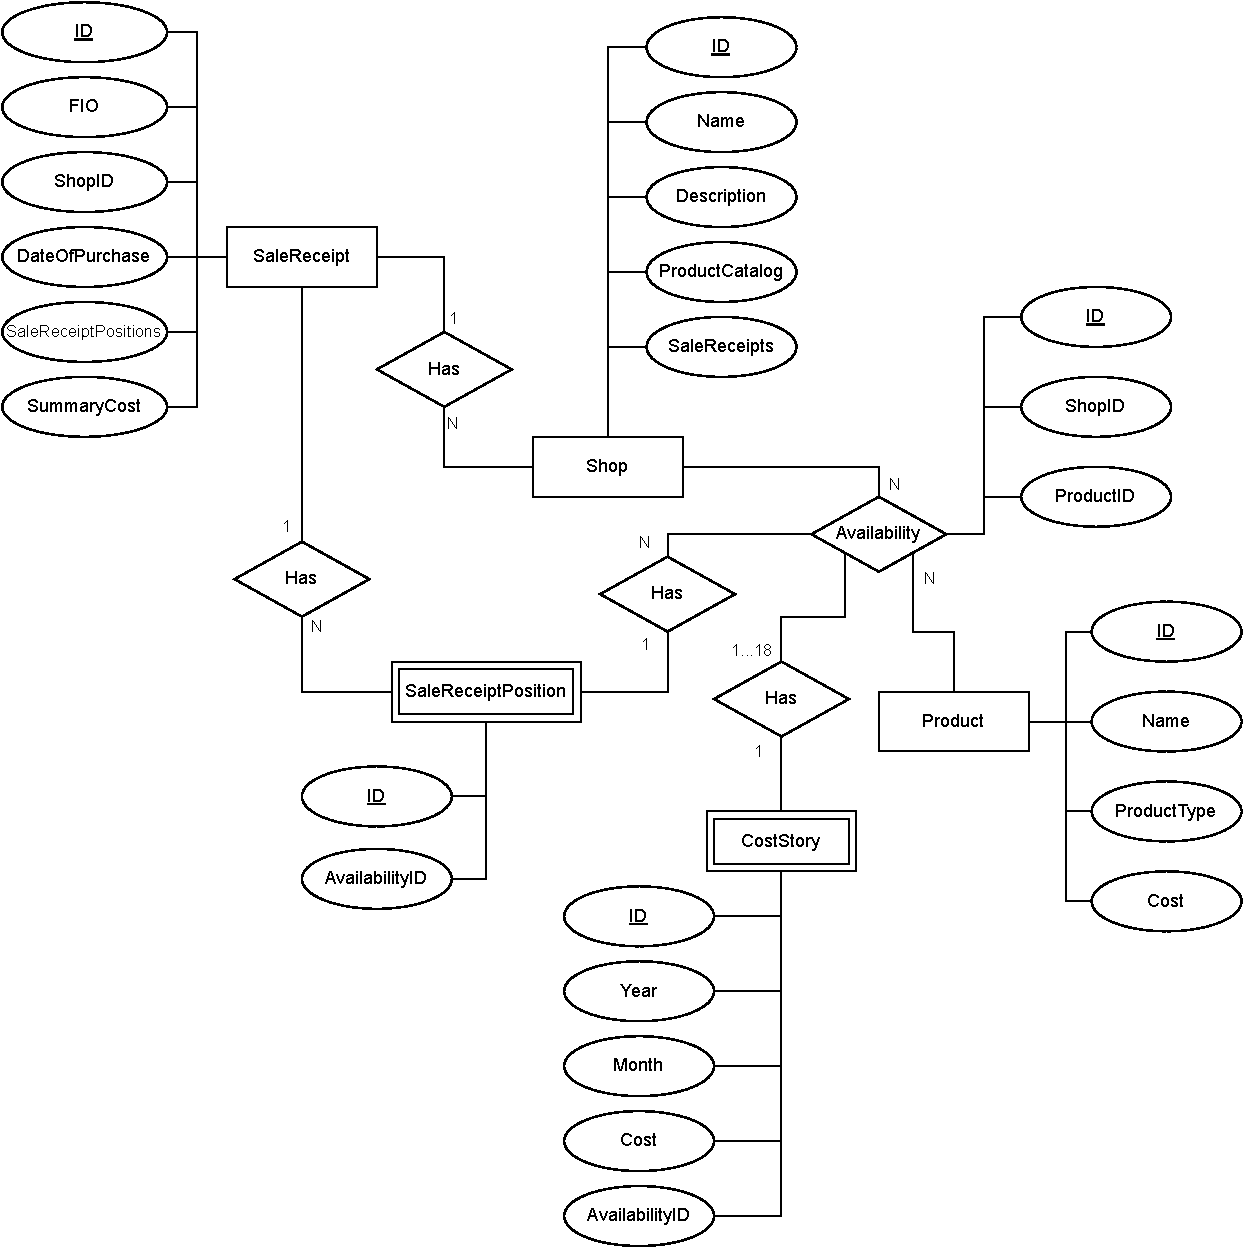
\includegraphics[scale=0.8]{ER.drawio.pdf}
	\caption{ER-диаграмма сущностей базы данных в нотации Чена.}
	\label{db_proj}
\end{figure}

\captionsetup[table]{skip=-12pt}
\captionsetup{singlelinecheck = false, justification=raggedright}
\begin{table}[H]
	\caption{Категории и описание данных}
	\begin{center}
		\begin{tabular}{| l | p{11 cm} |} 
			\hline
			
			\textbf{Категория} & \textbf{Описание} \\  
			
			\hline
			
			Магазин & Название, описание магазина, ассортимент товаров \\
			
			\hline
			
			Товар & Название, тип товара, актуальная цена \\
			
			\hline
			
			Ассортимент товаров & Список товаров \\
			
			\hline
			
			История цен & Год, месяц, цена в этот период \\
			
			\hline
			
			Товарный чек & ФИО, дата покупки, информация о месте покупки(магазине), список купленных товаров, итоговая стоимость \\
			\hline
		\end{tabular}
	\end{center}
\end{table}

\section{Описание ролевой модели}

Для управления системой введено три роли: пользователь, аналитик, администратор. На рисунке \ref{use_case} представлена Use-case-диаграмма ПО.

\captionsetup{singlelinecheck = false, justification=centering}
\begin{figure}[H]
	\centering
	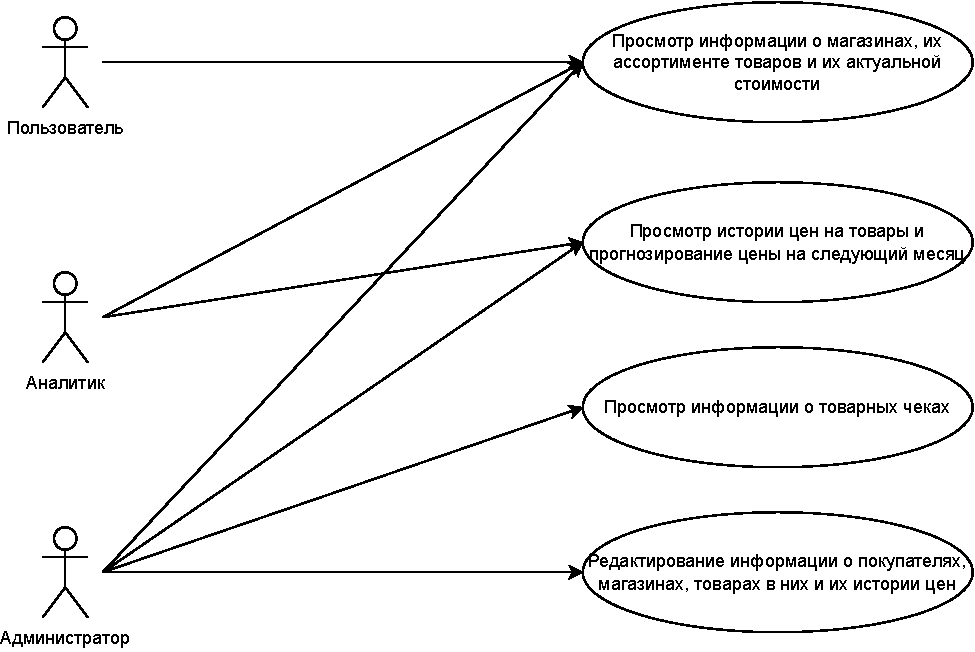
\includegraphics[scale=0.8]{use_case.drawio.pdf}
	\caption{Use-case-диаграмма ПО.}
	\label{use_case}
\end{figure}

\captionsetup{singlelinecheck = false, justification=raggedright}
\begin{table}[H]
	\caption{Роли и описание их функционала}
	\begin{center}
		\begin{tabular}{| l | p{12 cm} |} 
			\hline
			
			\textbf{Роль} & \textbf{Функционал} \\  
			
			\hline
			
			Пользователь & Просмотр информации о магазинах, их ассортименте товаров и их актуальной стоимости \\
			
			\hline
			
			Аналитик & Просмотр информации о магазинах, их ассортименте товаров и их истории цен. Возможность прогнозирования цены на товар в магазине \\
			
			\hline
			
			Администратор & Просмотр, добавление и удаление информации о магазинах, их ассортименте товаров и их истории цен, товарных чеках. Возможность прогнозирования цены на товар в магазине \\
			
			\hline
		\end{tabular}
	\end{center}
\end{table}

\captionsetup{singlelinecheck = false, justification=centering}

Для доступа к ролям <<Аналитик>> и <<Администратор>> требуется авторизация (ввод пароля).

\section{Обзор существующих СУБД}

Система управления базами данных (сокр. СУБД) -- Программная система, предназначенная для создания и хранения базы данных на основе некоторой модели данных, обеспечения логической и физической целостности содержащихся в ней данных, надежного и эффективного использования ресурсов (данных, пространства памяти и вычислительных ресурсов), предоставления к ней санкционированного доступа для приложений и конечных пользователей, а также для поддержки 
функций администратора базы данных \cite{kogal}.

""\newline
Функции СУБД:

\begin{itemize}
	\setlength\itemsep{0.01em}
	\item управление данными во внешней памяти;
	\item управление данными в оперативной памяти с использованием дискового кэша;
	\item журнализация изменений, резервное копирование и восстановление базы данных после сбоев;
	\item поддержка языков БД.
\end{itemize}

\subsection{Классификация СУБД по модели данных}

Модель данных --  система типов данных, типов связей между ними и допустимых видов ограничений целостности, которые могут быть для них определены. Здесь имеется в виду современное понимание типа данных как носителя свойств, определяющих и состояние экземпляров типа, и их поведение \cite{kogal}.

По этому признаку СУБД делят на:

\begin{itemize}
	\setlength\itemsep{0.01em}
	\item дореляционные;
	\item реляционные;
	\item постреляционные.
\end{itemize}


\subsection*{Дореляционные СУБД}

К ним относятся иерархические и сетевые СУБД.

""\newline
\noindent\textbf{Иерархические СУБД}

В иерархических СУБД используется представление базы данных в виде древовидной (иерархической) структуры, состоящей из объектов (данных) различных уровней.

Между объектами существуют связи, каждый объект может включать в себя несколько объектов более низкого уровня. Такие объекты находятся в отношении предка (объект более близкий к корню) к потомку (объект более низкого уровня), при этом возможна ситуация, когда объект-предок не имеет потомков или имеет их несколько, тогда как у объекта-потомка обязательно только один предок. Объекты, имеющие общего предка, называются близнецами \cite{scienceforum}.

Примеры: Caché, Google App Engine Datastore API.

""\newline
\noindent\textbf{Сетевые СУБД}

Сетевые СУБД подобны иерархическим, за исключением того, что в них имеются указатели в обоих направлениях, которые соединяют родственную информацию.

Несмотря на то, что эта модель решает некоторые проблемы, связанные с иерархической моделью, выполнение простых запросов остается достаточно сложным процессом.

Также, поскольку логика процедуры выборки данных зависит от физической организации этих данных, то эта модель не является полностью независимой от приложения. Другими словами, если необходимо изменить структуру данных, то нужно изменить и приложение \cite{scienceforum}.

Примеры: Caché.

\subsection*{Реляционные СУБД}

Реляционные СУБД ориентированы на организацию данных в виде двумерных таблиц. Каждая реляционная таблица представляет собой двумерный массив и обладает следующими свойствами:

\begin{enumerate}
	\setlength\itemsep{0.01em}
	\item каждый элемент таблицы является одним элементом данных;
	\item каждый столбец обладает своим уникальным именем;
	\item одинаковые строки в таблице отсутствуют;
	\item все столбцы в таблице однородные, то есть все элементы в столбце имеют одинаковый тип;
	\item порядок следования строк и столбцов может быть произвольным.
\end{enumerate}

Практически все разработчики современных приложений, предусматривающих связь с системами баз данных, ориентируются на реляционные СУБД. По оценке Gartner в 2013 году рынок реляционных СУБД составлял 26 млрд долларов с годовым приростом около 9\%, а к 2018 году рынок реляционных СУБД достигнет 40 млрд долларов. В настоящее время абсолютными лидерами рынка СУБД являются компании Oracle, IBM и Microsoft, с общей совокупной долей рынка около 90\%, поставляя такие системы как Oracle Database, IBM DB2 и Microsoft SQL Server \cite{dbms}.


\subsection*{Постреляционные СУБД}

Постреляционная модель является расширением реляционной модели. Она снимает ограничение неделимости данных, допуская многозначные поля, значения которых состоят из подзначений, и набор значений воспринимается как самостоятельная таблица, встроенная в главную таблицу \cite{post_rel}.

С ним относятся объектно-ориентированные и объектно-реляционные СУБД.

""\newline
\noindent\textbf{Объектно-ориентированные СУБД}

Объектно-ориентированные СУБД управляют базами данных, в которых данные моделируются в виде объектов, их атрибутов, методов и классов.

Этот вид СУБД позволяет работать с объектами баз данных так же, как с объектами в программировании в объектно-ориентированных языках программирования. ООСУБД расширяет языки программирования, прозрачно вводя долговременные данные, управление параллелизмом, восстановление данных, ассоциированные запросы и другие возможности  \cite{dbms}.

Примеры: GemStone.

""\newline
\noindent\textbf{Объектно-реляционные СУБД}

Объектно-реляционные СУБД поддерживают некоторые технологии, реализующие объектно-ориентированный подход: объекты, классы и наследование реализованы в структуре баз данных и языке запросов.

Зачастую все те СУБД, которые называются реляционными, являются, по факту, объектно-реляционными \cite{dbms}.

В данной работе будет рассмотрен имено этот класс СУБД.

Примеры: PostgreSQL, DB2, Oracle Database, Microsoft SQL Server.


\section{Методы построения линии тренда}

Линия тренда -- прямая или кривая линия, аппроксимирующая (приближающая) исходные данные на основе уравнения регрессии или скользящего среднего \cite{lt_exel}. Аппроксимация определяется по ме­тоду наименьших квадратов \cite{mnk}. В зависимости от характера поведения исходных данных (убыва­ют, возрастают и т.д.) выбирается метод интерполяции, который сле­дует использовать для построения тренда.

\subsection{Виды линий трендов}

\subsubsection*{Линейная линия тренда}

Линейная линия тренда определяется функцией

\begin{equation}
	y = ax + b,
\end{equation}

где $a$ -- тангенс угла наклона прямой, $b$ -- смещение.

Прямая линия тренда (линейный тренд) наилучшим образом подходит для величин, изменяющихся с постоянной скоростью. Приме­няется в случаях, когда точки данных расположены близко к прямой \cite{lt_exel}.

\subsubsection*{Логарифмическая линия тренда}

Логарифмическа линия тренда определяется функцией

\begin{equation}
	y = a\ln x + b,
\end{equation}

где $a$ и $b$ -- константы.

Логарифмическая линия тренда соответствует ряду данных, значения которого вначале быстро растут или убывают, а затем постепенно стабилизируются. Может использоваться для положительных и отрицательных данных \cite{lt_exel}.

\subsubsection*{Полиномиальная линия тренда}

Полиномиальная линия тренда определяется функцией

\begin{equation}
	y = \sum_{i = 0}^{n} a_i x^i, n \leqslant 6,
\end{equation}

где $a_i$ -- коэффициенты полинома.

Полиномиальная линия тренда используется для описания попеременно возрастающих и убывающих данных. Степень полинома подбирают таким образом, чтобы она была на единицу больше количества экстремумов (максимумов и минимумов) кривой \cite{lt_exel}.

\subsubsection*{Экспоненциальная линия тренда}

Экспоненциальная линия тренда определяется функцией

\begin{equation}
	y = a e ^ {bx},
\end{equation}

где $a$ и $b$ -- константы.

Экспоненциальный тренд используется в случае непрерывного возрастания изменения данных. Построение указанного тренда не­возможно, если в множестве значений членов ряда присутствуют нулевые или отрицательные данные \cite{lt_exel}.

\subsubsection*{Степенная линия тренда}

Степенная линия тренда определяется функцией

\begin{equation}
	y = a x ^ b,
\end{equation}

где $a$ и $b$ -- константы.

Степенная линия тренда дает хорошие результаты для положительных данных с постоянным ускорением. Для рядов с нулевыми или отрицательными значениями построение указанной линии трен­да невозможно \cite{lt_exel}.

\subsubsection*{Линейная фильтрация}

Линейная фильтрация определяется формулой

\begin{equation}
	F_t = \frac{A_t + A_{t-1} + ... + A_{t-n+1}}{n}, (2 \leqslant t < n),
\end{equation}

где $n$ -- общее число членов ряда, $t$ -- параметр фильтра.

Тренд с линейной фильтрацией позволяет сгладить колебания данных, наглядно демонстрируя характер зависимостей \cite{lt_exel}. Для построения указанной линии тренда пользователь должен задать число $t$.

Линейная фильтрация использует метод скользящего среднего, при котором каждое значение функции заменяется средним арифметическим $A$ по $t$ соседним точкам, расположенным симметрично относительно данной. Линия тренда в этом случае уравнения не имеет \cite{lin_filt}, поэтому для прогноза изменения величины она не подходит.

\subsection{Анализ исходных данных для построения линии тренда}

Цена товара как величина положительная и имеет непостоянный рост: она может как расти, так и падать. Таким образом, для прогнозирования цен на товары подходит полиномиальная линия тренда.

\section*{Вывод к аналитическому разделу}
\addcontentsline{toc}{section}{Вывод к аналитическому разделу}

В данном разделе были формализованы данные, хранимые в базе данных, описана ролевая модель, рассмотрены существующие СУБД и методы построения линии тренда.

\chapter{Конструкторский раздел}

В данном разделе представлена разработанная база данных для поставленной задачи, описаны объекты этой БД и ее система безопасности.

\section{Разработка базы данных}

В базе данных существует 6 таблиц, одна из которых является развязочной (Availability), и одно представление. Они представлены на диаграмме в виде сущностей. На рисунке \ref{db} представлена ER-диаграмма сущностей БД.

\begin{figure}[H]
	\centering
	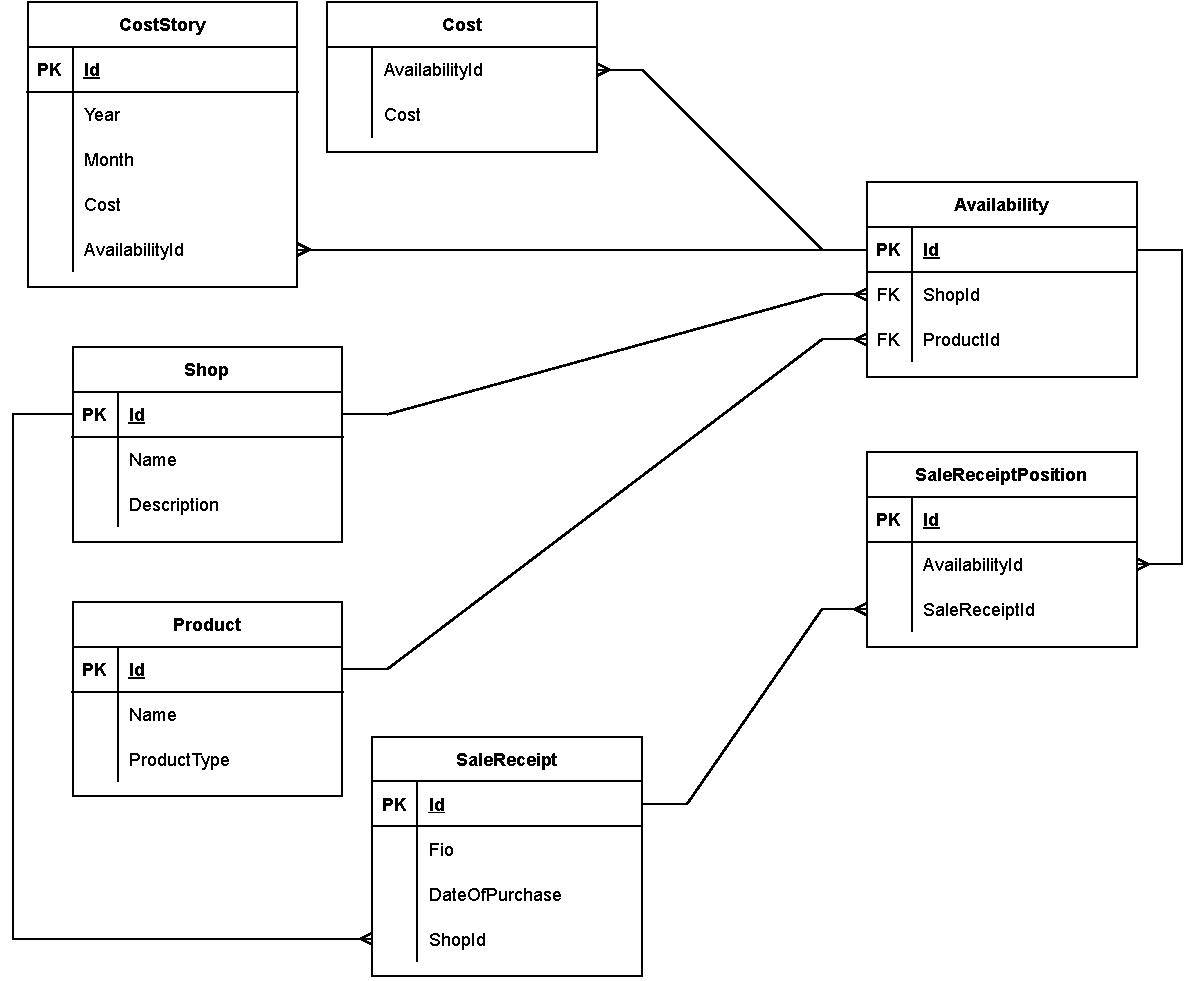
\includegraphics[scale=0.8]{ER-DB.drawio.pdf}
	\caption{ER-диаграмма сущностей БД.}
	\label{db}
\end{figure}

Таблица \textbf{Shop} хранит данные о магазинах и содержит следующие поля:
\begin{itemize}
	\setlength\itemsep{0.01em}
	\item ID -- идентификатор магазина;
	\item Name -- название магазина;
	\item Description -- описание магазина.
\end{itemize}

""\newline\indent
Таблица \textbf{Product} хранит данные о продуктах и содержит следующие поля:
\begin{itemize}
	\setlength\itemsep{0.01em}
	\item ID -- идентификатор продукта;
	\item Name -- название продукта;
	\item ProductType -- тип продукта.
\end{itemize}

""\newline\indent
Таблица \textbf{Availability} хранит отношения наличия товара в каталоге магазина и содержит следующие поля:
\begin{itemize}
	\setlength\itemsep{0.01em}
	\item ID -- идентификатор отношения;
	\item ShopID -- идентификатор магазина;
	\item ProductID -- идентификатор продукта.
\end{itemize}

""\newline\indent
Таблица \textbf{CostStory} хранит историю цен на товары в магазинах и содержит следующие поля:
\begin{itemize}
	\setlength\itemsep{0.01em}
	\item ID -- идентификатор значения цены в конкретный год и месяц;
	\item Year -- год;
	\item Month -- месяц;
	\item Cost -- значение цены в конкретный год и месяц;
	\item AvailabilityID -- идентификатор отношения наличия товара в каталоге магазина.
\end{itemize}

""\newline\indent
Представление \textbf{Cost} хранит актуальное значение цены на товар в магазине и содержит следующие поля:
\begin{itemize}
	\setlength\itemsep{0.01em}
	\item AvailabilityID -- идентификатор отношения наличия товара в каталоге магазина;
	\item Cost -- значение актуальной цены.
\end{itemize}

""\newline\indent
Таблица \textbf{SaleReceipt} хранит данные о товарных чеках и содержит следующие поля:
\begin{itemize}
	\setlength\itemsep{0.01em}
	\item ID -- идентификатор товарного чека;
	\item FIO -- ФИО покупателя;
	\item ShopID -- идентификатор магазина, в котором была совершена покупка;
	\item DateOfPurchase -- дата покупки.
\end{itemize}

""\newline\indent
Таблица \textbf{SaleReceiptPosition} хранит информацию о позиции в чеке и содержит следующие поля:
\begin{itemize}
	\setlength\itemsep{0.01em}
	\item ID -- идентификатор позиции чека;
	\item AvailabilityID -- идентификатор отношения наличия товара в каталоге магазина.
\end{itemize}

""\newline\indent
Таблицы \textbf{SaleReceiptPosition} и \textbf{CostStory} содержат поле идентификатора отношения наличия товара в каталоге магазина в целях борьбы с рассинхронизацией: товарный чек и история цен на товар в магазине не могут ссылаться на товары, которых нет в данном магазине.

Актуальная стоимость товара в магазине формируется как последнее по дате значение цены товара в истории цен.

\section{Разработка объектов базы данных}

Для разработанной базы данных были созданы 4 хранимые функции на выборку и триггер для обновления истории цен. Далее представлены их реализации и описание.

\captionsetup{singlelinecheck = false, justification=raggedright}
\begin{lstlisting}[language=sql, caption={Реализация хранимой функции get\_products\_by\_shopid}]
create or replace function get_products_by_shopid(shop_id integer)
returns table(ProdID integer, ProdName text, ProdType text, Cost float)
as $$
	select APC.ProductID, APC.Name, APC.ProductType, APC.Cost
	from (((select Availability.ID as AvailID, Availability.ShopID, Availability.ProductID from Availability where Availability.ShopID = shop_id) as A 
	join Products on A.ProductID = Products.ID) as AP join Costs on AP.AvailID = Costs.AvailabilityID) as APC;
$$ language sql;
\end{lstlisting}

""\newline\indent
Функция \textbf{get\_products\_by\_shopid} возвращает список товаров, продающиеся в указанном магазине с идентификатором shop\_id. 

""\newline
\begin{lstlisting}[language=sql, caption={Реализация хранимой функции get\_coststory\_by\_shopid\_prodid}]
create or replace function get_coststory_by_shopid_prodid(shop_id integer, prod_id integer)
returns table(Year integer, Month integer, Cost integer)
as $$
	select CostStory.Year, CostStory.Month, CostStory.Cost
	from CostStory
	where AvailabilityID = (select ID
	from Availability
	where ShopID = shop_id and ProductID = prod_id);
$$ language sql;
\end{lstlisting}

""\newline\indent
Функция \textbf{get\_coststory\_by\_shopid\_prodid} предназначена для поиска полной истории цен на указанный товар в указанном магазине посредством их идентификаторов prod\_id и shop\_id соответственно.

\begin{lstlisting}[language=sql, caption={Реализация хранимой функции get\_salereceipts\_by\_shopid}]
create or replace function get_salereceipts_by_shopid(shop_id integer)
returns table(SR_ID integer, FIO text, DateOfPurchase date, SummaryCost integer)
as $$
	select S.S_ID, max(FIO), max(DateOfPurchase), sum(Cost) as SummaryCost
	from ((select ID as S_ID, FIO, ShopID, DateOfPurchase from SaleReceipts where ShopID = shop_id) as SR join SaleReceiptPositions on SaleReceiptPositions.SaleReceiptID = SR.S_ID) as S join Costs on S.AvailabilityID = Costs.AvailabilityID
	group by S.S_ID;
$$ language sql;
\end{lstlisting}

""\newline\indent
Функция \textbf{get\_salereceipts\_by\_shopid} возвращает список товарных чеков в указанном магазине посредством его идентификатора shop\_id. 
\newpage
\begin{lstlisting}[language=sql, caption={Реализация хранимой функции get\_content\_from\_salereceipt}]
create or replace function get_content_from_salereceipt(sr_id integer)
returns table(ProdID integer, Name text, ProductType text, Cost integer)
as $$
	select SAP.ProductID as ProdID, Name, ProductType, Cost::integer
	from ((SaleReceiptPositions join Availability on SaleReceiptPositions.AvailabilityID = Availability.ID) as SA join Products on Products.ID = SA.ProductID) as SAP join Costs on SAP.AvailabilityID = Costs.AvailabilityID
	where SaleReceiptID = sr_id;
$$ language sql;
\end{lstlisting}

""\newline\indent
Функция \textbf{get\_content\_from\_salereceipt} возвращает список товаров товарного чека с идентификатором sr\_id. 

Сценарий создания всей базы данных (вместе с триггером) расположен в Приложении А.

\section{Разработка системы безопасности БД}

В соответствии с описанной в Аналитическом разделе ролевой моделью, были созданы три пользователя с различными уровнями доступа к данным в БД.

\begin{itemize}
	\item <<Пользователь>>: имеет доступ только на чтение к таблицам магазинов Shops, товаров Products, стоимостей Costs и отношения наличия Availability.
	\item <<Аналитик>>: имеет доступ только на чтение к таблицам магазинов Shops, товаров Products, стоимостей Costs, истории цен на товары в магазинах CostStory и отношения наличия Availability.
	\item <<Администратор>>: имеет доступ ко всем таблицам БД с наличием прав на редактирование информации в них.
\end{itemize}

Как было сказано в Аналитическом разделе, для доступа к ролям <<Аналитик>> и <<Администратор>> требуется авторизация (ввод пароля).

\section*{Вывод к конструкторскому разделу}
\addcontentsline{toc}{section}{Вывод к конструкторскому разделу}

В данном разделе была представлена разработанная база данных для поставленной задачи, описаны объекты этой БД и ее система безопасности.

\chapter{Технологический раздел}

В данном разделе представлены средства реализации и интерфейс программного обеспечения.

\section{Средства реализации}

\subsection*{Обзор и выбор СУБД}

Для выбора СУБД формулируются следующие критерии:

\begin{itemize}
	\item открытость;
	\item поддержка хранимых процедур и триггеров;
	\item кроссплатформенность;
	\item поддержка БД неограниченного размера;
\end{itemize}

Далее представлена таблица сравнения рассматриваемых СУБД по заданным критериям \cite{orc_db, mssql, pg, db2}.

\captionsetup{singlelinecheck = false, justification=raggedright}
\begin{table}[H]
	\caption{Сравнение СУБД по критериям}
	\begin{center}
		\begin{tabular}{| p{5 cm} | c | c | c | c |} 
			\hline
			
			\textbf{} & \textbf{Oracle DB} & \textbf{SQL Server} & \textbf{DB2} & \textbf{PostgreSQL} \\  
			
			\hline
			
			Открытость & - & - & - & + \\
			
			\hline
			
			Поддержка хранимых процедур и триггеров & + & + & - & + \\
			
			\hline
			
			Кроссплатформенность & + & - & + & + \\
			
			\hline
			
			Поддержка БД неограниченного размера & + & - & - & + \\
			
			\hline
		\end{tabular}
	\end{center}
\end{table}

Основываясь на таблице сравнения СУБД, для решения задачи была выбрана СУБД PostgreSQL.

\subsection*{Выбор и обснование средств реализации ПО}

В качестве языка программирования для реализации программного обеспечения для работы с БД был выбран C\# \cite{c_sharp}. Выбор этого языка обусловлен тем, что он обладает удобным синтаксисом, управляемым кодом и сборщиком мусора, благодаря этому не нужно заботится об утечках памяти, об указателях и о некоторых базовых структурах и алгоритмах -- все это уже реализовано. Это позволит ускорить разработку и отладку кода. Также данный язык предоставляет большую часть требуемого функционала для решения поставленной задачи, для недостающего функционала существует связанным с ним пакетным менеджер NuGet \cite{nuget}.

Для разработки пользовательского интерфейса программного обеспечения была выбрана платформа WPF \cite{wpf}. Данная платформа обладает декларативным определением элементов интерфейса с помощью языка разметки XAML \cite{xaml}, независимостью от разрешения экрана. Это значит, что приложение будет корректно масштабироваться под разные экраны с разным разрешением, а также данный интерфейс не будет жёстко зависеть от логики программы.

В качестве среды разработки (IDE) была выбрана Visual Studio \cite{vs}, обладающая интеллектуальными подсказками, инструментами анализа, отладки и тестирования кода, поставляющаяся вместе с языком C\# и пакетным менеджером NuGet.

\section{Интерфейс ПО}

Интерфейс включает в себя 4 секции для работы с БД.

\begin{enumerate}
	\setlength\itemsep{0.01em}
	\item Работа с магазинами.
	\item Работа с товарами магазинов.
	\item Работа с товарными чеками магазинов.
	\item Работа с историей цен товаров в магазинах.
\end{enumerate}

""\newline\indent
На рисунках \ref{ui1}-\ref{ui3} продемонстрирована работоспособность программы.
\captionsetup{singlelinecheck = false, justification=centering}
\begin{figure}[H]
	\centering
	\frame{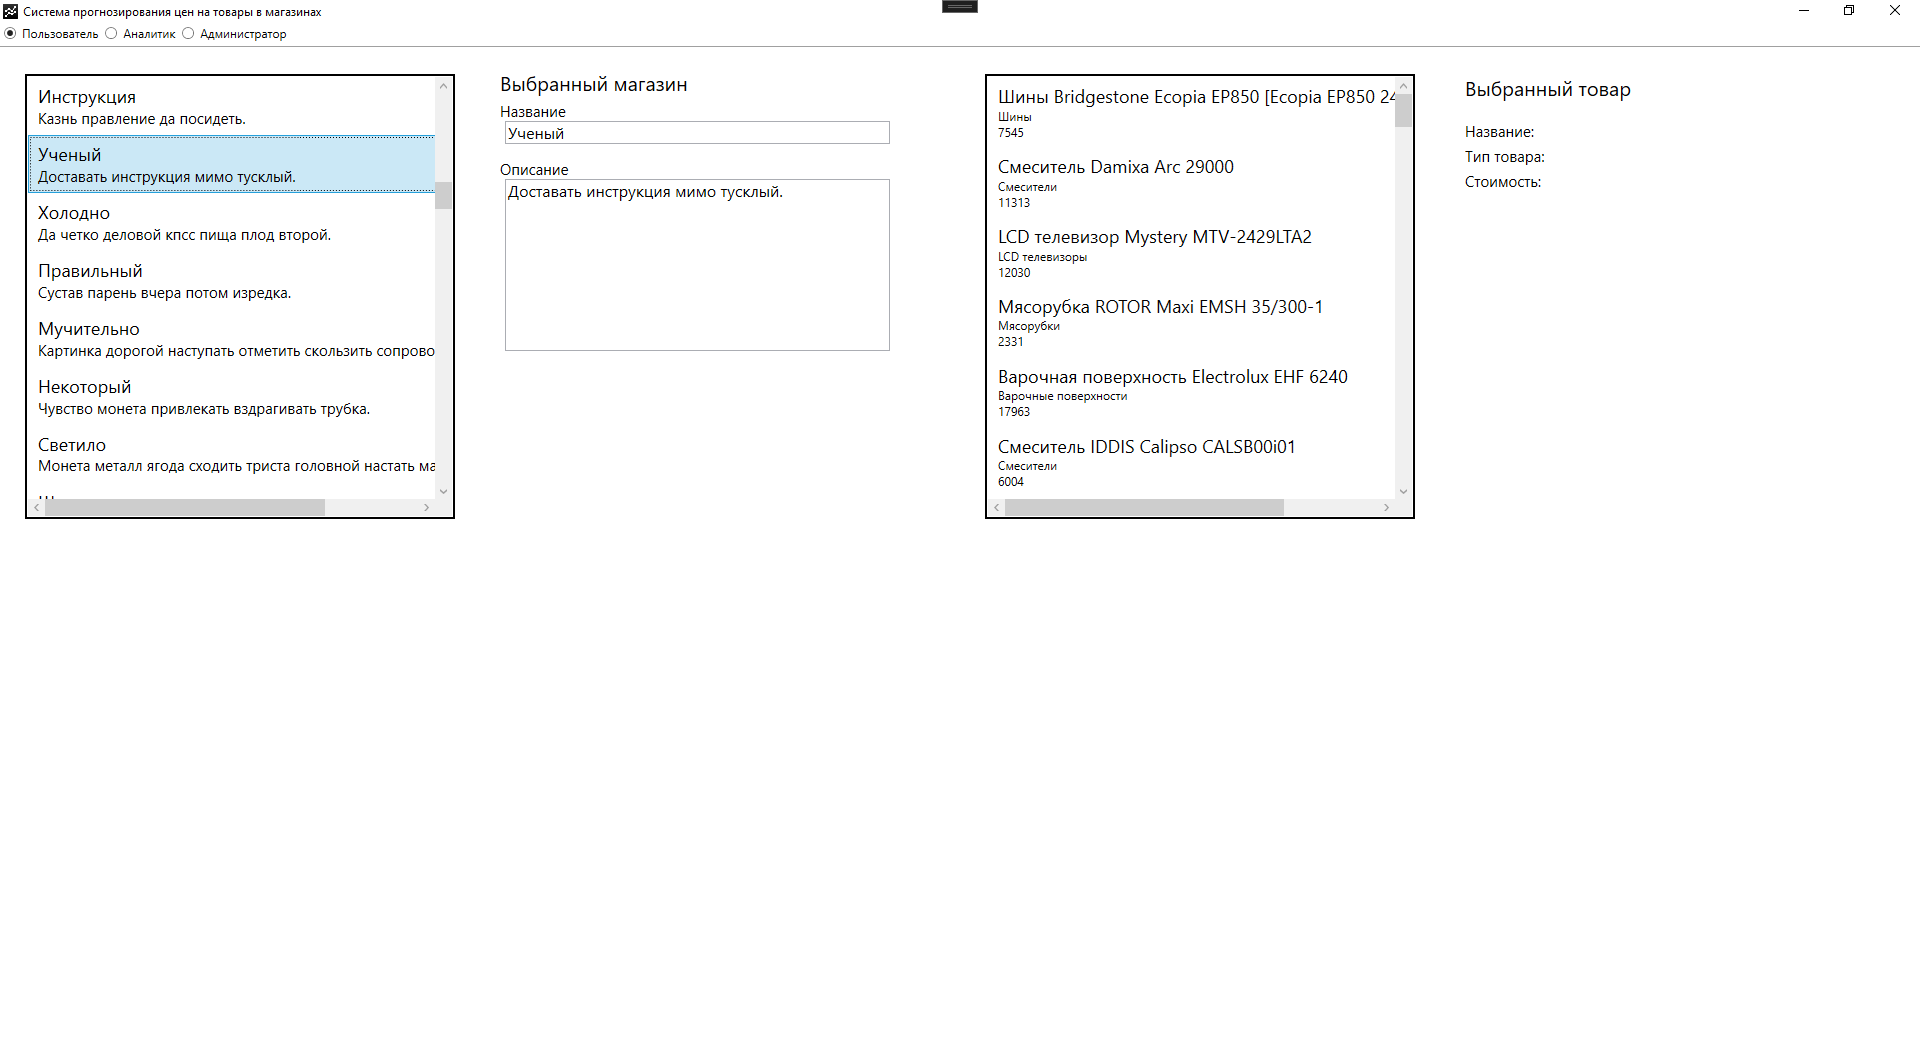
\includegraphics[scale=0.325]{ui_user.png}}
	\caption{Работа приложения в режиме пользователя.}
	\label{ui1}
\end{figure}

\begin{figure}[H]
	\centering
	\frame{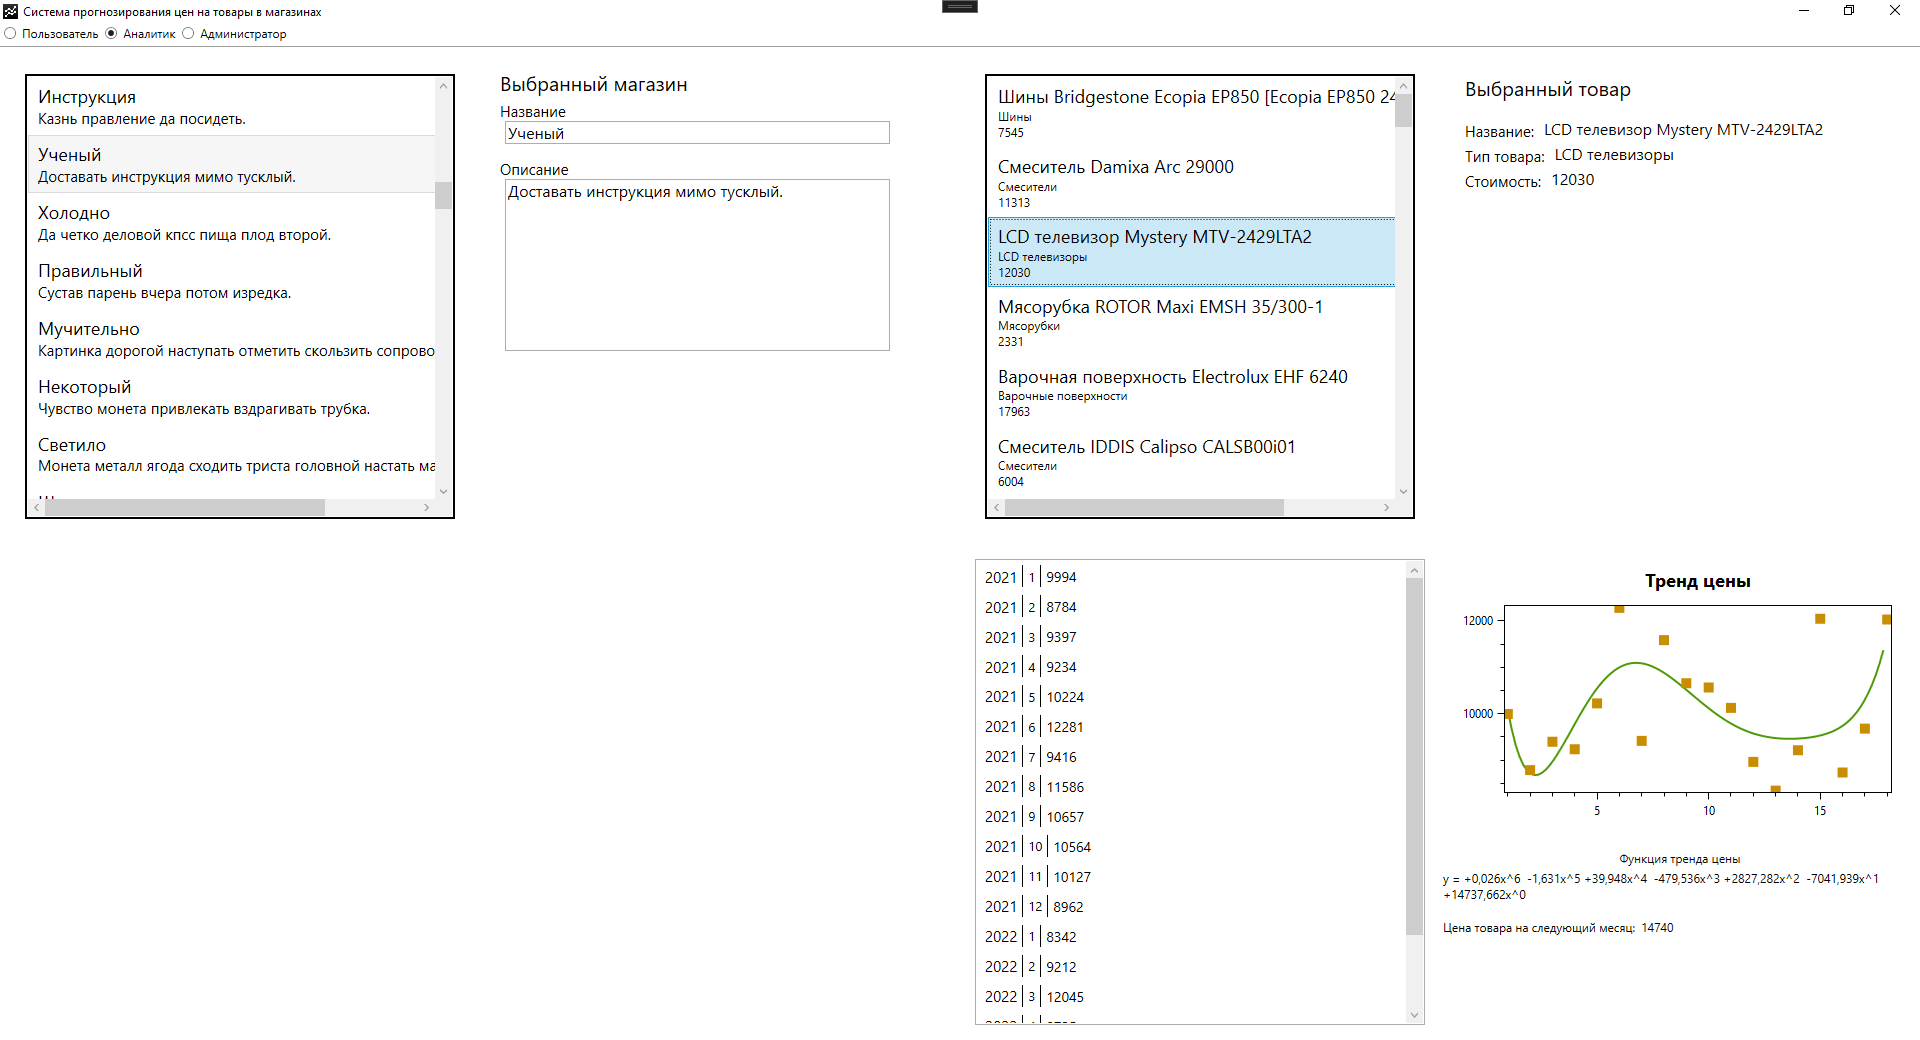
\includegraphics[scale=0.325]{ui_analyst.png}}
	\caption{Работа приложения в режиме аналитика.}
	\label{ui2}
\end{figure}

\begin{figure}[H]
	\centering
	\frame{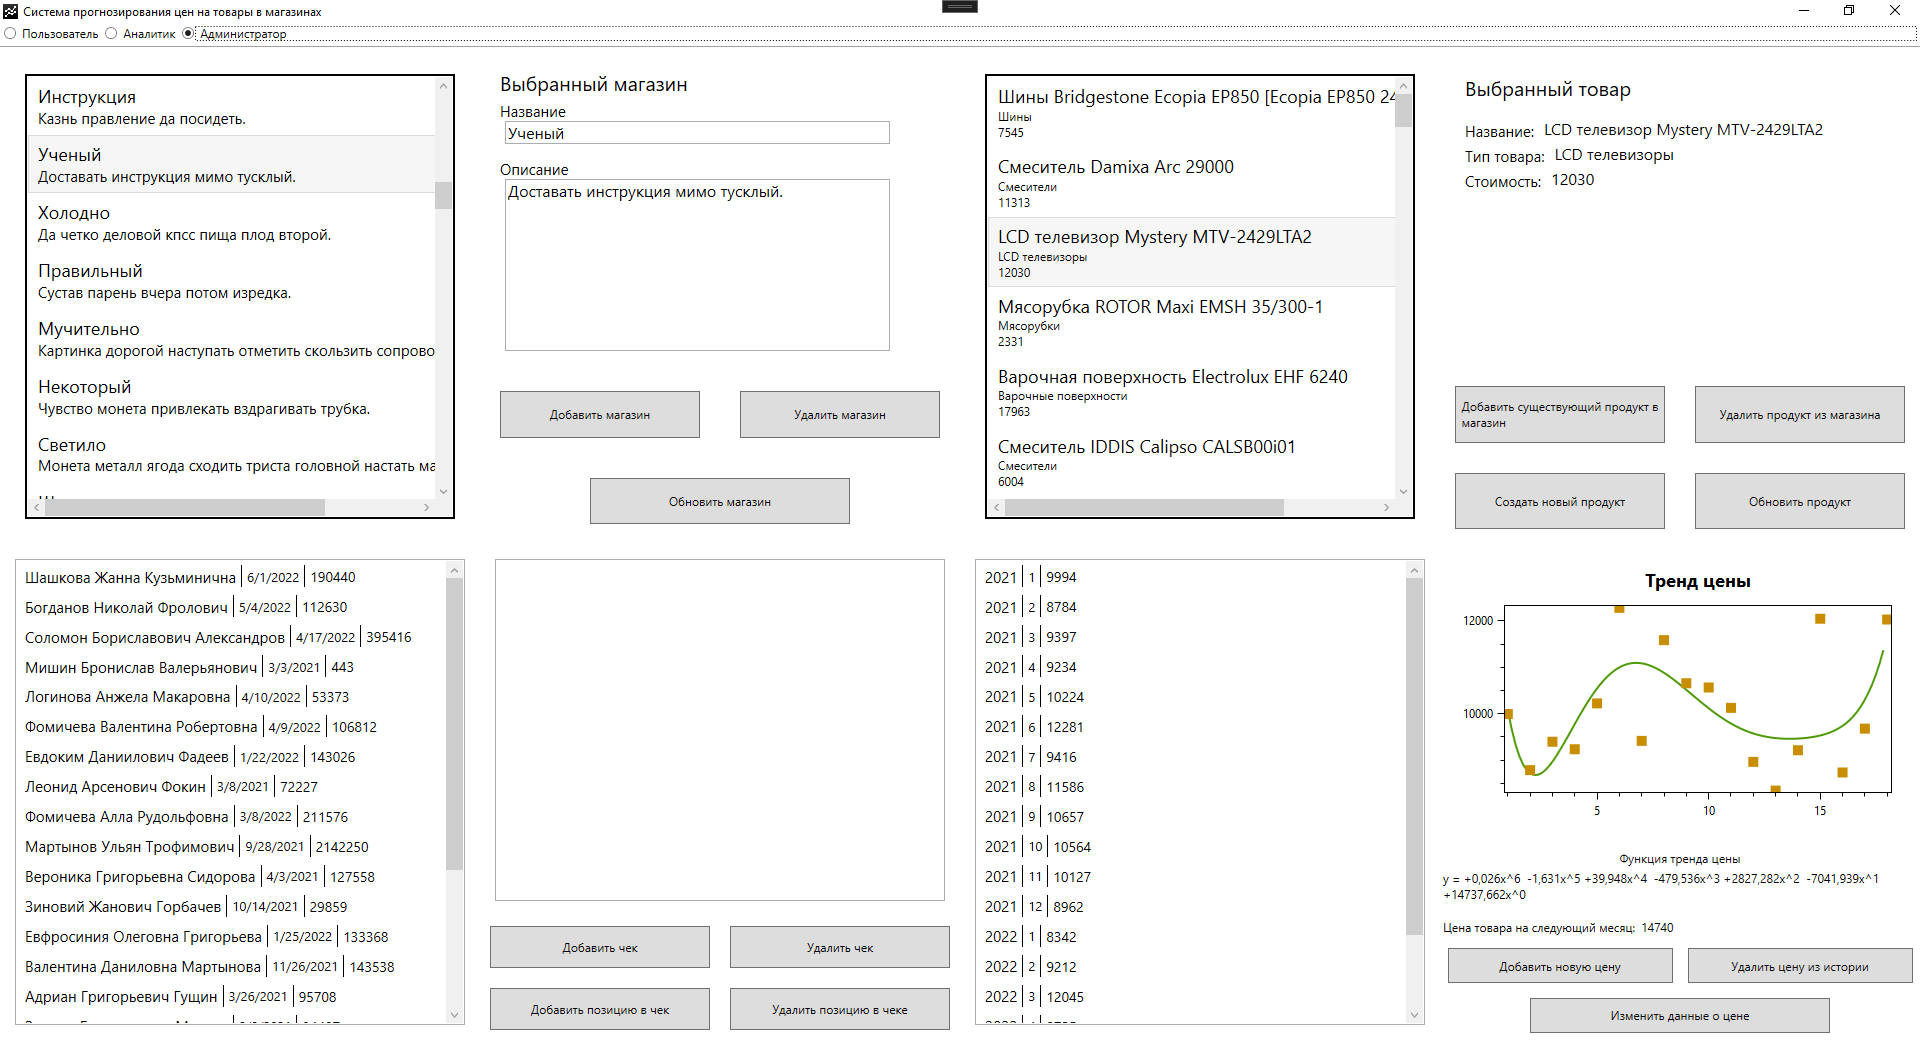
\includegraphics[scale=0.325]{ui_admin.png}}
	\caption{Работа приложения в режиме администратора.}
	\label{ui3}
\end{figure}

\section*{Вывод к технологическому разделу}
\addcontentsline{toc}{section}{Вывод к технологическому разделу}

В данном разделе были представлены средства реализации и интерфейс программного обеспечения.

\chapter{Экспериментальный \newline раздел}

В данном разделе поставлен эксперимент по оценке отклонения значения стоимости товара на следующий месяц при неполной выборке истории цен от реального значения стоимости товара на следующий месяц.

\section{Постановка эксперимента}

\subsection{Цель эксперимента}

Целью эксперимента является проведение анализа отклонения значения стоимости товара на следующий месяц при неполной выборке истории цен от реального значения стоимости товара на следующий месяц.

\subsection{Описание эксперимента}

В данном эксперименте был выбран товар с указанной в таблице 4.1 историей цен. Далее при расчете очередного значения стоимости товара на следующий месяц при неполной выборке истории цен объем выборки будет ограничиваться от 1 до $N = 18$, где $N$ -- объем полной выборки.

\captionsetup{singlelinecheck = false, justification=raggedright}
\begin{table}[H]
	\caption{История цен выбранного для эксперимента товара}
	\begin{center}
		\begin{tabular}{| c | c | c |} 
			\hline
			
			\textbf{Год} & \textbf{Месяц} & \textbf{Цена} \\  
			
			\hline
			
			2021 & 1 & 16883 \\
			
			\hline
			
			2021 & 2 & 17283 \\
			
			\hline
			
			2021 & 3 & 15860 \\
			
			\hline
			
			2021 & 4 & 17194 \\
			
			\hline
			
			2021 & 5 & 20262 \\
			
			\hline
			
			2021 & 6 & 16655 \\
			
			\hline
			
			2021 & 7 & 16983 \\
			
			\hline
			
			2021 & 8 & 13709 \\
			
			\hline
			
			2021 & 9 & 19365 \\
			
			\hline
			
			2021 & 10 & 17504 \\
			
			\hline
			
			2021 & 11 & 18579 \\
			
			\hline
			
			2021 & 12 & 14264 \\
			
			\hline
			
			2022 & 1 & 14831 \\
			
			\hline
			
			2022 & 2 & 19490 \\
			
			\hline
			
			2022 & 3 & 16791 \\
			
			\hline
			
			2022 & 4 & 22657 \\
			
			\hline
			
			2022 & 5 & 21632 \\
			
			\hline
			
			2022 & 6 & 18796 \\
			
			\hline
		\end{tabular}
	\end{center}
\end{table}

\section{Результаты экперимента}

В результате эксперимента были получены значения, представленные в таблице 4.2, где

\begin{itemize}
	\item n -- количество используемых значений для вычисления стоимости товара на следующий месяц;
	\item $\hat{y}$ -- аппроксимированное значение стоимости товара на следующий месяц;
	\item $y$ -- реальное значение стоимости товара на следующий месяц;
	\item $\sqrt{\frac{(\hat{y} - y) ^ 2}{y ^ 2}}$ -- среднее значение относительной погрешности.
\end{itemize}

\begin{table}[H]
	\caption{Результаты эксперимента}
	\begin{center}
		\begin{tabular}{| c | c | c | c |} 
			\hline
			
			\textbf{n = 1..N} & \textbf{$\hat{y}$} & \textbf{$y$} & \textbf{$\sqrt{\frac{(\hat{y} - y) ^ 2}{y ^ 2}}$, \%} \\  
			
			\hline
			1 & 16883 & 17283 & 2,31 \\
			\hline
			2 & 17283 & 15860 & 8,97 \\
			\hline
			3 & 15859 & 17194 & 7,76 \\
			\hline
			4 & 17194 & 20262 & 15,14 \\
			\hline
			5 & 20342 & 16655 & 22,13 \\
			\hline
			6 & 16662 & 16983 & 1,89 \\
			\hline
			7 & 16952 & 13709 & 23,65 \\
			\hline
			8 & 13735 & 19365 & 29,07 \\
			\hline
			9 & 19292 & 17504 & 10,21 \\
			\hline
			10 & 17560 & 18579 & 5,48 \\
			\hline
			11 & 18296 & 14264 & 28,26 \\
			\hline
			12 & 14155 & 14831 & 4,55 \\
			\hline
			13 & 14549 & 19490 & 25,35 \\
			\hline
			14 & 19561 & 16791 & 16,49 \\
			\hline
			15 & 17579 & 22657 & 22,41 \\
			\hline
			16 & 22544 & 21632 & 4,21 \\
			\hline
			17 & 22183 & 18796 & 18,01 \\
			\hline
			18 & 18939 & 18796 & 0,76 \\
			\hline
		\end{tabular}
	\end{center}
\end{table}

\section*{Вывод к экспериментальному разделу}
\addcontentsline{toc}{section}{Вывод к экспериментальному разделу}

В данном разделе был поставлен эксперимент по оценке отклонения значения стоимости товара на следующий месяц при неполной выборке истории цен от реального значения стоимости товара на следующий месяц.

Из результатов эксперимента видно, что иногда ошибка не превышает 5\%, а иногда превышает более 15\%, что говорит о некачественности модели. Можно сделать вывод о том, что использование полинома шестой степени для предсказания следующего значения на основе предыдущих не всегда является лучшим решением: несмотря на большую степень полинома, которая увеличивает точность аппроксимации, то есть уменьшает сумму квадратов, ошибка возрастает из-за наличия больших флуктуаций между точками.


\chapter*{Заключение}
\addcontentsline{toc}{chapter}{Заключение}

В ходе выполнения курсового проекта были формализованы данные, хранимые в базе данных, описана ролевая модель, рассмотрены существующие СУБД и методы построения линии тренда. Была представлена разработанная база данных для поставленной задачи, описаны объекты этой БД и ее система безопасности. Также были представлены средства реализации и интерфейс программного обеспечения для выполнения данной задачи.

Созданная база данных позволяет хранить информацию о магазинах, товарах в них, товарных чеках и их содержимом, а также истории цен на товары в магазинах. Созданный программный продукт для работы с базой данных позволяет работать с информацией из нее: просматривать, добавлять, редактировать, удалять, анализировать.

Также был поставлен эксперимент, в ходе которого были выявлены изъяны модели для предсказания стоимости товара на основе полинома n-ой степени.

В качестве развития проекта можно предложить реализацию более качественных моделей для прогнозирования стоимостей товаров на следующий месяц для лучшей аппроксимации цены на товар в магазине. 

\newpage
\addcontentsline{toc}{chapter}{Список литературы}
\renewcommand\bibname{Список литературы}

\begin{thebibliography}{3}
	\bibitem{hse_pred} Методы и модели социально-экономического прогнозирования : учебник и практикум для академического бакалавриата. В 2-х т. Т. 1. Теория и методология прогнозирования / И. С. Светуньков, С. Г. Светуньков. — М. : Издательство Юрайт, 2014. — 351 с. — Серия : Бакалавр. Академический курс.
	
	\bibitem{bel_prog} Касперович С.А. Прогнозирование и планирование экономики : курс лекций для студентов специальностей 1-25 01 07 «Экономика и управление предприятием», 1-25 01 08 «Бухгалтерский учет, анализ и аудит», 1-26 02 02 «Менеджмент», 1-26 02 03 «Маркетинг» / С. А. Касперович. - Минск. : БГТУ, 2007. - 172 с. 
	
	\bibitem{met_pred_online} К. В. Богданов. Методика прогнозирования цен на товары в интернет-магазинах [Электронный ресурс]. -- Режим доступа: https://cyberleninka.ru/article/n/metodika-prognozirovaniya-tsen-na-tovary-v-internet-magazinah/viewer (дата обращения 4.04.2022)
	
	\bibitem{kogal} Когаловский М.Р. Энциклопедия технологий баз данных. — М.: Финансы и статистика, 2002. — 800 с.
	
	\bibitem{scienceforum} Классификация систем управления базами данных [Электронный ресурс]. -- Режим доступа: https://scienceforum.ru/2016/article/2016019197 (дата обращения 6.04.2022)
	
	\bibitem{dbms} Системы управления базами данных [Электронный ресурс]. -- Режим доступа: https://lecturesdb.readthedocs.io/databases/dbms.html (дата обращения 8.04.2022)
	
	\bibitem{post_rel} Постреляционная, многомерная и объектно-ориентированная модели данных [Электронный ресурс]. -- Режим доступа:  http://bseu.by/it/tohod/lekcii2\_4.htm?ysclid=l3njaseoko (дата обращения 8.04.2022)
	
	\bibitem{lt_exel} Построение линии тренда в Excel [Электронный ресурс]. -- Режим доступа: https://ya-znau.ru/znaniya/zn/202 (дата обращения 9.04.2022)
	
	\bibitem{mnk} Линник Ю. В. Метод наименьших квадратов и основы математико-статистической теории обработки наблюдений. — 2-е изд. — М., 1962. (математическая теория)
	
	\bibitem{lin_filt} Линейная фильтрация [Электронный ресурс]. -- Режим доступа: https://poznayka.org/s23136t1.html (дата обращения 9.04.2022)
	
	\bibitem{orc_db} Oracle Database [Электронный ресурс]. -- Режим доступа: https://www.oracle.com/database/ (дата обращения 12.04.2022)
	
	\bibitem{mssql} Microsoft SQL-Server  [Электронный ресурс]. -- Режим доступа:  https://www.microsoft.com/ru-ru/sql-server/sql-server-2019 (дата обращения 12.04.2022)
	
	\bibitem{pg} PostgreSQL [Электронный ресурс]. -- Режим доступа: https://www.postgresql.org/ (дата обращения 12.04.2022)
	
	\bibitem{db2} DB2 [Электронный ресурс]. -- Режим доступа: https://www.ibm.com/analytics/db2 (дата обращения 12.04.2022)
	
	\bibitem{c_sharp} Документация по C\# [Электронный ресурс]. -- Режим доступа: https://docs.microsoft.com/ru-ru/dotnet/csharp/ (дата обращения 14.04.2022)
	
	\bibitem{nuget} NuGet [Электронный ресурс]. -- Режим доступа: https://www.nuget.org/ (дата обращения 14.04.2022)
	
	\bibitem{wpf} Что такое Windows Presentation Foundation (WPF)? [Электронный ресурс]. -- Режим доступа:  https://docs.microsoft.com/ru-ru/visualstudio/designers/getting-started-with-wpf?view=vs-2022 (дата обращения 14.04.2022)
	
	\bibitem{xaml} Обзор XAML (WPF .NET) [Электронный ресурс]. -- Режим доступа:  https://docs.microsoft.com/ru-ru/dotnet/desktop/wpf/xaml/?view=netdesktop-6.0 (дата обращения 14.04.2022)
	
	\bibitem{vs} Visual Studio [Электронный ресурс]. -- Режим доступа:  https://visualstudio.microsoft.com/ru/ (дата обращения 14.04.2022)
\end{thebibliography}

\chapter*{Приложение А}

\begin{lstlisting}[language=sql, caption={Реализация триггера для обновления истории цен}]
create or replace function remove_too_old_coststory()
returns trigger
as $$
	declare
		old_date_id integer;
		old_date date;
		new_date_id integer;
		new_date date;
		months_diff integer;
		new_avail_id integer;
	begin
		new_avail_id := new.AvailabilityID;
		

		select min(make_date(prod_coststory.Year, prod_coststory.Month, 1)) into old_date
		from (select * 
		from CostStory 
		where AvailabilityID = new_avail_id) as prod_coststory;
		
		select prod_coststory.id into old_date_id
		from (select * 
		from CostStory 
		where AvailabilityID = new_avail_id) as prod_coststory
		where make_date(prod_coststory.Year, prod_coststory.Month, 1) = old_date;
		

		select max(make_date(prod_coststory.Year, prod_coststory.Month, 1)) into new_date
		from (select * 
		from CostStory 
		where AvailabilityID = new_avail_id) as prod_coststory;
		
		select prod_coststory.id into new_date_id
		from (select * 
		from CostStory 
		where AvailabilityID = new_avail_id) as prod_coststory
		where make_date(prod_coststory.Year, prod_coststory.Month, 1) = new_date;
		
		select (date_part('year', new_date) - date_part('year', old_date)) * 12 + (date_part('month', new_date) - date_part('month', old_date)) + 1
		into months_diff;
		
		if months_diff > 18 then
		delete from CostStory where AvailabilityID = new_avail_id and ID = old_date_id;
		end if;
		return new;
	end
$$ language plpgsql;

drop trigger update_coststory on CostStory;
create trigger update_coststory after insert on CostStory
for each row execute function remove_too_old_coststory();
\end{lstlisting}

\begin{lstlisting}[language=sql, caption={Сценарий создания БД}]
Drop database if exists spsr_lt_db;
Create database spsr_lt_db;

create table Shops
(
	ID serial primary key,
	Name text not null,
	Description text not null
);

create table SaleReceipts
(
	ID serial primary key,
	FIO text not null,
	ShopID integer not null,
	DateOfPurchase date not null,
	foreign key (ShopID) references Shops(ID) on delete cascade
);

create table Products
(
	ID serial primary key,
	Name text not null,
	ProductType text not null
);

create table Availability
(
	ID serial primary key,
	ShopID integer not null,
	ProductID integer not null,
	foreign key (ShopID) references Shops(ID) on delete cascade,
	foreign key (ProductID) references Products(ID) on delete cascade
);

create table SaleReceiptPositions
(
	ID serial primary key,
	AvailabilityID integer not null,
	SaleReceiptID integer not null,
	foreign key (AvailabilityID) references Availability(ID) on delete cascade,
	foreign key (SaleReceiptID) references SaleReceipts(ID) on delete cascade
);

create table CostStory
(
	ID serial primary key,
	Year integer not null,
	Month integer not null,
	Cost integer not null,
	AvailabilityID integer not null,
	foreign key (AvailabilityID) references Availability(ID) on delete cascade
);

create view Costs as
	select T.AvailabilityID, Cost
	from CostStory join (select AvailabilityID, max(make_date(Year, Month, 1)) as CostDate
	from CostStory
	group by AvailabilityID) as T on T.AvailabilityID = CostStory.AvailabilityID and T.CostDate = make_date(CostStory.Year, CostStory.Month,1);


create or replace function remove_too_old_coststory()
returns trigger
as $$
	declare
		old_date_id integer;
		old_date date;
		new_date_id integer;
		new_date date;
		months_diff integer;
		new_avail_id integer;
	begin
		new_avail_id := new.AvailabilityID;
		

		select min(make_date(prod_coststory.Year, prod_coststory.Month, 1)) into old_date
		from (select * 
		from CostStory 
		where AvailabilityID = new_avail_id) as prod_coststory;
		
		select prod_coststory.id into old_date_id
		from (select * 
		from CostStory 
		where AvailabilityID = new_avail_id) as prod_coststory
		where make_date(prod_coststory.Year, prod_coststory.Month, 1) = old_date;
		

		select max(make_date(prod_coststory.Year, prod_coststory.Month, 1)) into new_date
		from (select * 
		from CostStory 
		where AvailabilityID = new_avail_id) as prod_coststory;
		
		select prod_coststory.id into new_date_id
		from (select * 
		from CostStory 
		where AvailabilityID = new_avail_id) as prod_coststory
		where make_date(prod_coststory.Year, prod_coststory.Month, 1) = new_date;
		
		select (date_part('year', new_date) - date_part('year', old_date)) * 12 + (date_part('month', new_date) - date_part('month', old_date)) + 1
		into months_diff;
		
		if months_diff > 18 then
		delete from CostStory where AvailabilityID = new_avail_id and ID = old_date_id;
		end if;
		return new;
	end
$$ language plpgsql;

drop trigger update_coststory on CostStory;
create trigger update_coststory after insert on CostStory
for each row execute function remove_too_old_coststory();

create user "user";
grant connect on database spsr_lt_db to "user";
grant usage on schema public to "user";
grant select on table Shops, Products, Availability, Costs to "user";
alter user "user" with password 'user';

create user "analyst" with password 'analyst';
grant connect on database spsr_lt_db to "analyst";
grant usage on schema public to "analyst";
grant select on table Shops, Products, Availability, CostStory to "analyst";
grant select on table Costs to "analyst";

create user "admin" with password 'admin';
grant connect on database spsr_lt_db to "admin";
grant usage on schema public to "admin";
grant select, insert, update, delete on all tables in schema public to "admin";

drop user if exists "user";
drop user if exists "analyst";
drop user if exists "admin";

create or replace function get_products_by_shopid(shop_id integer)
returns table(ProdID integer, ProdName text, ProdType text, Cost float)
as $$
	select APC.ProductID, APC.Name, APC.ProductType, APC.Cost
	from (((select Availability.ID as AvailID, Availability.ShopID, Availability.ProductID from Availability where Availability.ShopID = shop_id) as A 
	join Products on A.ProductID = Products.ID) as AP join Costs on AP.AvailID = Costs.AvailabilityID) as APC;
$$ language sql;

create or replace function get_coststory_by_shopid_prodid(shop_id integer, prod_id integer)
returns table(Year integer, Month integer, Cost integer)
as $$
	select CostStory.Year, CostStory.Month, CostStory.Cost
	from CostStory
	where AvailabilityID = (select ID
	from Availability
	where ShopID = shop_id and ProductID = prod_id);
$$ language sql;

create or replace function get_salereceipts_by_shopid(shop_id integer)
returns table(SR_ID integer, FIO text, DateOfPurchase date, SummaryCost integer)
as $$
	select S.S_ID, max(FIO), max(DateOfPurchase), sum(Cost) as SummaryCost
	from ((select ID as S_ID, FIO, ShopID, DateOfPurchase from SaleReceipts where ShopID = shop_id) as SR join SaleReceiptPositions on SaleReceiptPositions.SaleReceiptID = SR.S_ID) as S join Costs on S.AvailabilityID = Costs.AvailabilityID
	group by S.S_ID;
$$ language sql;

create or replace function get_content_from_salereceipt(sr_id integer)
returns table(ProdID integer, Name text, ProductType text, Cost integer)
as $$
	select SAP.ProductID as ProdID, Name, ProductType, Cost::integer
	from ((SaleReceiptPositions join Availability on SaleReceiptPositions.AvailabilityID = Availability.ID) as SA join Products on Products.ID = SA.ProductID) as SAP join Costs on SAP.AvailabilityID = Costs.AvailabilityID
	where SaleReceiptID = sr_id;
$$ language sql;


copy Products from '...\tables_data\Products.csv' delimiter ';' CSV HEADER;
copy Shops from '...\tables_data\Shops.csv' delimiter ';' CSV HEADER;
copy SaleReceipts from '...\tables_data\SaleReceipts.csv' delimiter ';' CSV HEADER;
copy Availability from '...\tables_data\Availability.csv' delimiter ';' CSV HEADER;
copy SaleReceiptPositions from '...\tables_data\SaleReceiptPositions.csv' delimiter ';' CSV HEADER;
copy CostStory from '...\tables_data\CostStory.csv' delimiter ';' CSV HEADER;
\end{lstlisting}

\end{document}